\documentclass[12pt]{article}
\usepackage[margin=1in]{geometry}
\usepackage[T1]{fontenc}
\usepackage{mathptmx}
\usepackage[parfill]{parskip}
%\usepackage{amsmath}
\usepackage{graphicx}
%\usepackage{listings}   % allows lstlisting environment
%\usepackage{moreverb}   % allows listinginput environment
%\usepackage{siunitx}
%\usepackage{enumerate}
%\usepackage{epstopdf}
%\usepackage{booktabs}
%\usepackage{float}
%\usepackage{multirow}
%\usepackage{mhchem}
%\usepackage{lscape}
\usepackage{hyperref}
\hypersetup{
    colorlinks=true,
    linkcolor=blue,
    filecolor=magenta,      
    urlcolor=cyan,
}

\newcommand{\horrule}[1]{\rule{\linewidth}{#1}} % Create horizontal rule command with 1 argument of height

\newcommand\mytitle{Evolution 3\\Compsci 458}
\title{\horrule{5pt}\\\vspace{0.4cm}{\bf \mytitle}\\}
\author{Jiawei Zhang, Davis Treybig, Michael Han, and Kevin Do}
\date{\horrule{1pt}}

\begin{document}
\maketitle{}
\section{Summary}
\begin{figure}[h]
\begin{center}
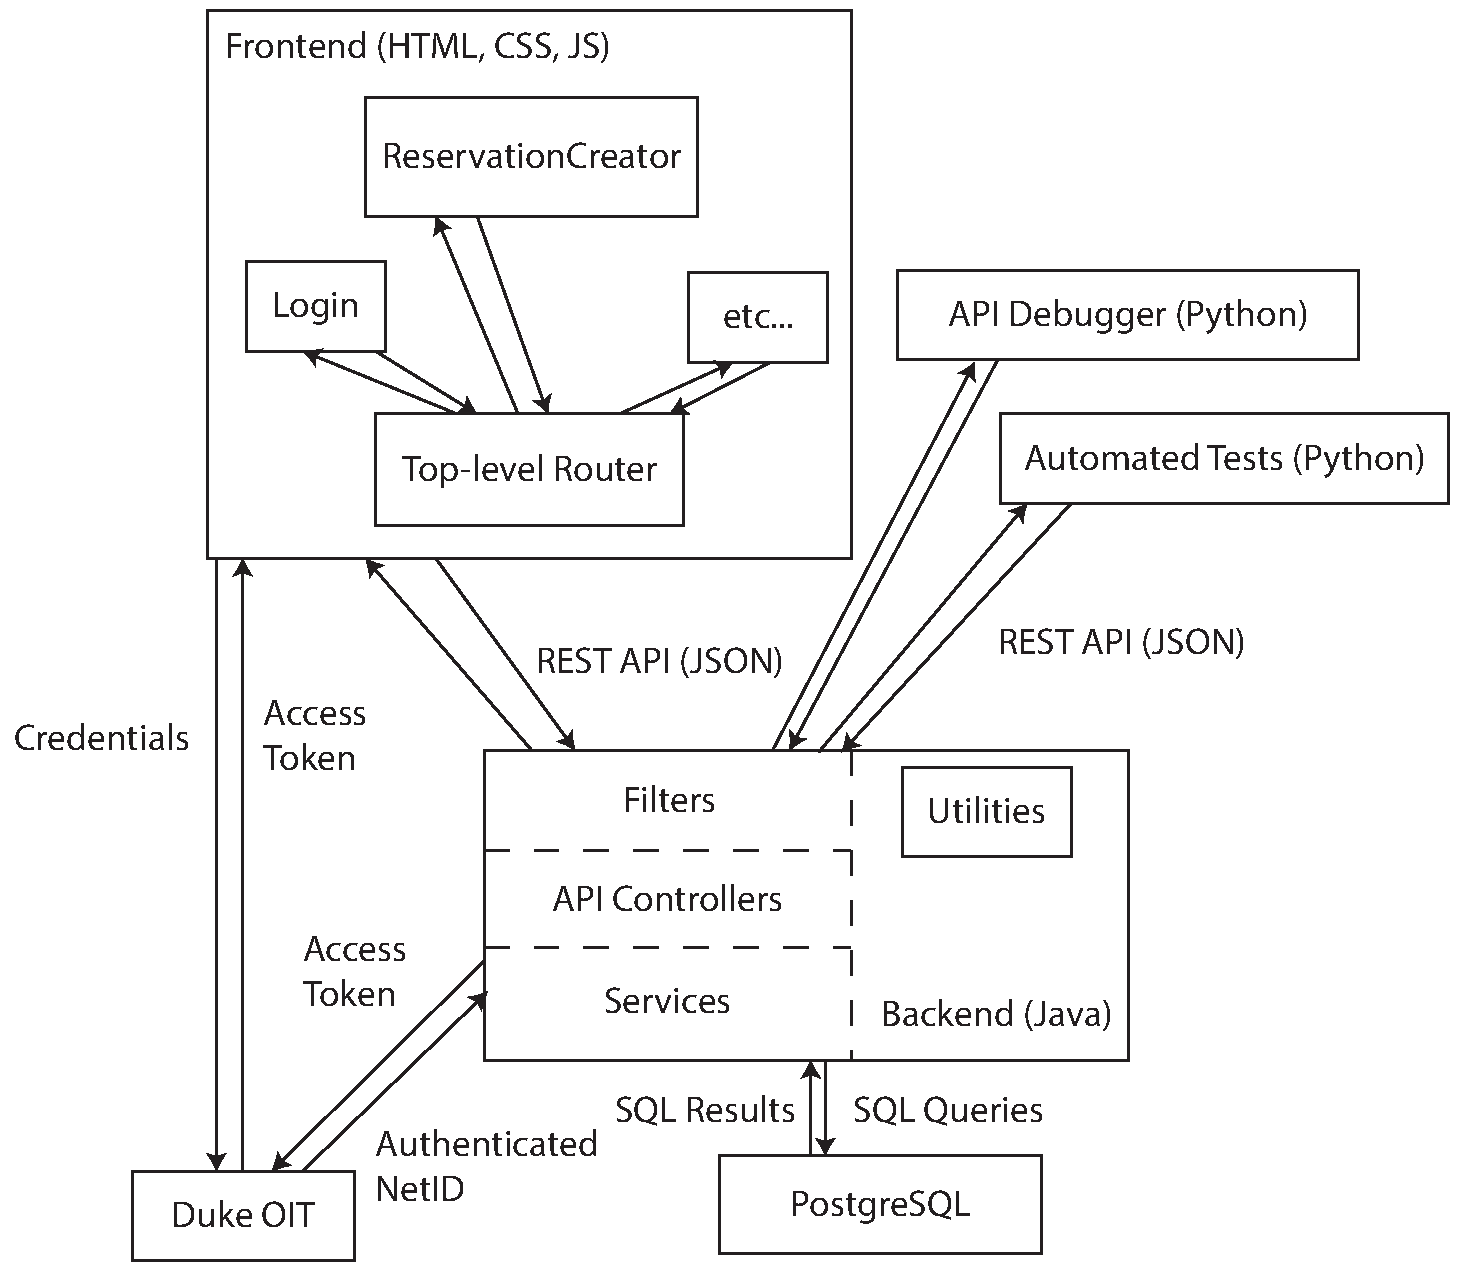
\includegraphics[height=4in]{../ev2/ev2_design_cropped.pdf}
\end{center}
\caption{Diagram of system architecture}
\label{fig:design}
\end{figure}

Our resource management tool is a web application that uses the following technology stack: a React.js frontend, a Java Spring server, and a PostgreSQL database. In addition, we use Python scripts to automate the testing of our API. Our overall technology stack, as well as our overall code structure, have not changed since evolution 2. The primary changes are {\huge TODO}.

The rest of the changes required for evolution 3 fit nicely into our existing frameworks. In the backend, permissions were handled with a few new API calls on top of our evolution 1 API calls, and a few new DB tables were added to support these calls. {\huge TODO EXPAND IF NECESSARY}

For retrospectives on our former backend choices and more detail about our backend additions, see the \hyperref[sec:Backend]{backend section}. For retrospectives on our former frontend choices and more detail about our frontend additions, see the \hyperref[sec:Frontend]{frontend section}. Finally, see \hyperref[appendix:backendtest]{Appendix \ref{appendix:backendtest}} for our updated backend test strategy,  \hyperref[appendix:frontendtest]{Appendix \ref{appendix:frontendtest}} for our updated frontend test strategy, \hyperref[appendix:apispec]{Appendix \ref{appendix:apispec}} for our updated API specification, and \hyperref[appendix:DBDesign]{Appendix \ref{appendix:DBDesign}} for our updated database design. 

\section{Backend}
{\huge SOMEWHERE TALK ABOUT TYPE CHECKING DIFFICULTIES}

\label{sec:Backend}
The backend consists of the parts of the software system that run on a VPS (Virtual Private Server) using Ubuntu Linux 14.04. Our software uses PostgreSQL 9.5 for persistent data storage and the Java Spring Framework as the container for a Tomcat web server. If the backend were viewed as an MVC (Model-View-Controller), PostgreSQL would be the model and Java Spring would be the view (REST API) and the controller (request processing, database communication, and response creation). 

This architecture has not changed since evolution 2, and it has suited us well. 

\subsection{Java}
Java has continued to suit us well in evolution 3, and from a design perspective it did not significantly affect any of the evolution 3 requirements. Familiarity with Java has made development easy, and static typing has helped prevent bugs and improve code readability.

\subsection{Java Spring}
Spring has also continued to suit us well in evolution 3. Adding a new set of endpoints to handle incomplete reservations was extremely easy. Furthermore, as our codebase has gotten more and more complex, we have appreciated the structure that Spring enforces. This structure (an MVC structure based around services, controllers, filters, and utilities) has in effect ensured that our overall package and class layout is understandable, maintainable, and very extensible. 

\subsection{PostgreSQL}
\subsubsection{Retrospective}
PostgreSQL served us well for evolution 3. While perhaps more planning and setup was required for us to alter our DB schema from evolution 2 to evolution 3 than for a team using a NoSQL DB, we ultimately felt that this was a small amount of work. Furthermore, the result of such planning was a very clearly defined DB schema that made it easy for everyone (particularly those working on the backend) to understand how we were going to store data and therefore how to structure new endpoint code. Thus, we ultimately felt that having a structured DB improved our coding efficiency. 

In regards to choosing PostgreSQL over some other SQL DB, we have not needed to interact with the DB in such a way that some other SQL DB would have provided us better tools than PostgreSQL. Thus, we are still totally happy with PostGreSQL as a DB. 

\subsubsection{Current Design}
The following changes were made to our DB schema for evolution 2:
{\huge TODO UPDATE THE ENUMERATE BELOW}
\begin{enumerate}
    \item A title and description field were added to the Reservations table
    \item The "resource" column was removed from the reservations table, and instead we created a reservation-resources table. This was done because now each reservation can have multiple resources. This table also stores a "resource_approved" field to indicate which resources are approved for each reservation. 
    \item A "complete" boolean was added to the reservations table, to indicate which reservations are incomplete and which are not
\end{enumerate}

You can see a full diagram of this updated schema in  \hyperref[appendix:DBDesign]{Appendix \ref{appendix:DBDesign}}. 

\subsection{Security}
\subsubsection{Retrospective}
{\huge TODO UPDATE}
Our old security framework remained intact while tacking on Duke Shibboleth. We declined to use the tokens provided by Duke Shibboleth as they were undocumented and uncustomizable. 

\subsubsection{Current Design}
{\huge TODO UPDATE}
Evolution 2 introduced integration with Duke Shibboleth as a new requirement. We decided to keep our existing JSON web token (JWT) authentication framework and simply add Duke OAuth2 to our login. 

The evolution 2 spec requires that the old login stay intact for the admin, so we simply added a new button on the login page that redirected the user to a Duke-based authentication server. Depending on whether the user successfully authenticates using his or her NetID, the Duke server routes the user to a 'success' endpoint or a 'failure' endpoint. The failure endpoint is essentially the resource planner login page (with an added error message), while the success endpoint is a new endpoint which verifies the authcode returned by the Duke server using another Duke service. If this verification is successful, the user is logged in and given a JWT and directed to a page inside the resource manager. If this verification fails, the user is again redirected to the resource manager login. 

One major difference with the introduction of Duke Shibboleth authentication is the lack of user registration, since users can no longer be created by the admin. Instead, a user is 'created' the first time he or she logs into the resource planner. Besides the hashing and salting of the admin password, there is also no more password storage in our database as the resource planner no longer handles authentication directly, instead allowing Duke Shibboleth to simply pass us to an authcode after a successful user login that we can verify to ensure the user is valid. 

Upon login, a JSON Web Token (JWT) is generated, which stores the User ID and permission level of the logged-in user. This JWT, which is signed by a secret key known only to the server, authenticates future API calls without accessing the database. Instead of a database lookup, the authenticity of the JWT is confirmed using the secret key, and the User ID and permissions stored in the JWT can be used directly. 

For encrypting the communication between the client and the server, we decided to go with SSL as Spring provided support for it. We used Java's built in keytool to generate a Java keystore and self-signed certificate using RSA algorithm. We used a self-signed certificate rather than one signed by a legitimate CA because it was free. We also made it so that it can run on both HTTP and HTTPS at the same time for ease of testing. Non-SSL HTTP support can easily be disabled with a global switch.


\subsection{Testing}
\subsubsection{Retrospective}
{\huge TODO UPDATE}
For evolution 1 backend testing, we used a suite of API tests ran from a series of Python scripts. This strategy worked extremely well for us - by having a set of tests which covered the vast majority of API cases, we could quickly make changes and verify that nothing was broken. We stand by our decision to focus on testing only the API contract, and not the backend internals, because ultimately the API is what must be working for the web application to work correctly. Realistically, any major bug in the internals of the backend should affect the API tests as well.


Now, there as some exceptions to this. For instance, email is be very hard to test via Python scripts, and so our testing suite does not fully cover email. Similarly, since it is nearly impossible for an API testing suite to be 100 percent comprehensive, there are potentially situations where a backend bug would not break any tests, but would affect the web application. Nevertheless, we feel the chances of such issues occurring is so low that they are not worth worrying about. Given the fact that our presentation for evolution 1 had no issues and that our evolution 1 passed all grader test cases, we still feel quite confident in this strategy. 

We also stand by our decision to use Python, as Python scripts are simple to write and can be run quickly. In addition, our Python testing framework  \texttt{unittest} has proven very easy to use, and Python has numerous libraries that allow you to easily send HTTP requests. 

\subsubsection{Current Design}
{\huge TODO UPDATE}
For Evolution 2, we updated the test cases to reflect the new permissions, groups, and login protocol with NetID requirements. We added separate tests for groups and permissions but also integrated the new requirements into the existing tests, updating them as needed. In addition, we created the API Debugger which allows for easy testing of the endpoints. For simplicity, while we allow testing of the login endpoint, we run the other endpoint tests as admin. We chose to use the token from the admin because a basic debugger should show that the endpoints accomplish the tasks that they are designed for and not focus so much on who is trying to accomplish the tasks. The API debugger was also written in Python due to ease of sending requests and testing via \texttt{unittest}. 

We chose to not implement every test case in \hyperref[appendix:backendtest]{Appendix \ref{appendix:backendtest}} for backend testing because we felt that the current tests gave a fairly comprehensive view of functionality. That said, we did manually test all of the cases listed there.


\subsection{Code Structure}
\subsubsection{Retrospective}
Our code structure has essentially stayed the same for evolution 3. In evolution 2, we changed our overall code hierarchy to be divided into modules for each set of endpoints, and within each module we placed the different MVC pieces that related to that module. For instance, within the Reservation module, we placed our reservation controller, our reservation service, all reservation data structures, etc. We did this in order to ensure that our code was appropriately compartmentalized, such that someone who, for instance, needs to modify resource code, knows exactly where the relavent classes are. We are still very happy with this decision - it has made updating and modifying code in the backend much cleaner (for instance, instead of sifting through 20+ different custom data structures when making changes, you can go through the exact 3-4 relavent ones). 

Since many of the new requirements in evolution 3 were extensions of previous work (modifications to reservations, modifications to permissions, modifications to email), we did not have to add any significant new modules or classes. Rather, most of our work for evolution 3 involved slightly modifying or extending previously created controllers and services. 

\subsection{Current Design}
We have no plans to modify the aforementioned code structure, as it has suited us well and helped us maintain clean code at a high level in the backend. 


\subsection{Email}
\label{sec:EMAIL}
\subsubsection{Retrospective}
Our original design to handle emails sent at the start and end of reservations was as follows:
\begin{enumerate}
    \item An EmailService class was used to handle scheduling emails. This class kept track of queued emails to be sent in the future, and provided a simple API that could be called on reservation creation/modification/deletion to update queued email times, or add new emails to the queue, or delete queued emails.
    \item An EmailScheduler class, which handled the logic of actually composing the email, based on certain input parameters. This class would define the subject of each email, as well as its content. 
    \item An EmailUtility class, which handled the actually email API we use to send emails. 
\end{enumerate}

The basic workflow of the above was, individual service classes would call EmailService, EmailService would call EmailScheduler, and EmailScheduler would call EmailUtility. We felt this overall design was simple, easy to use, and quite extensible to future email requirements. 

\subsubsection{Retrospective and Current Design}
Evolution 3 introduced a number of new email requirements. Luckily, our original email scheduling design made adhering to these new requirements easy. Specifically, we only add to do the following things:
\begin{enumerate}
    \item We added a few new methods to EmailService to handle instantly-sent emails (such as an email for when an  incomplete reservation gets denied or canceled). These are all just 3-4 lines, and call EmailScheduler the same way former EmailService methods did. 
    \item We modified the API of EmailService slightly so that it would automatically detect what type of reservation was being scheduled for an email. Based on this info (complete reservation vs incomplete reservation), we alter the content of potential future emails, but all scheduling is done the exact same way as before. 
    \item We added a number of new potential input parameters to EmailScheduler, to handle the various new kinds of emails we need to send (reservation denied, reservation canceled, reservation about to be canceled, etc). 
    \item EmailUtility did not change at all. 
\end{enumerate}

Essentially, none of our old code had to change, none of our scheduling algorithms had to change, and we just had to add a few new types of emails and appropriately check for which type should be sent. As such, we are very happy with how we originally designed emails, and believe our current email code will continue to serve us well in the face of future changes. 


\subsection{Permissions}
\subsubsection{Retrospective And Current Design}
The permissions design we implemented for evolution 2 had two key factors:
\begin{enumerate}
    \item Storing resource-specific permissions as a single integer value (no access as 0, view access as 1, reserve access as 2), rather than as separate boolean values or values stored in separate DB tables. 
    \item Having all permission modification and viewing being done through a single permission matrix. 
\end{enumerate}

These design choices have proven to be very helpful. First of all, as we argued in our evolution 2 document, the choice to have all permissions be in a single place (the permission matrix) has made using and testing our system exceptionally easy. As we add new features and need to manually test them, we can trivially edit the permissions in the system to create the test scenario that we want to create. Had we separated out user permissions and group permissions or resource permissions and system permissions, it would have substantially slowed our manual testing and general usage of our application. 

Secondly, and more importantly, these design choices made it very easy to handle the new permission requirements for evolution 3. Evolution 3's major permission change is that there are now "resource managers". Our design enabled us to just define the standard that resource manager is represented by a value of 3 in our resource-specific permission tables. In other words, nothing in the backend had to change to handle resource managers being shown in the permission matrix or to handle resource managers being set via the permission matrix. 

In addition, new backend methods to retrieve resource managers (for the new incomplete reservation endpoints) were able to re-use much of our previous permission code, since detecting of resource managers involves all the same DB calls, but is simply checking for a different integer. 

As such, we feel that our argument in the evolution 2 doc that our permission design allowed the easy addition of new permissions has been shown as very true. Furthermore, we believe that if evolution 4 brings on even more permission variations, we should be able to easily accomodate those as well. 



\subsubsection{Assumptions}
Given the ambiguity of some evolution requirements, here are some of the assumptions we made this evolution:
\begin{enumerate}
    \item We assume that any person or any group that is a resource manager of a given resource also has both view and reserve permission for that resource. We confirmed this was a reasonable assumption via both Peter and Professor Hilton. 
    \item The evolution requirements state that an email must be sent warning a user that their upcoming incomplete reservation might get canceled if it is not approved in time. The time before the reservation that this email must be sent is unclear, however. We choose to send this email 10 minutes before the scheduled start time. 
    \item It is somewhat unclear in the guidelines which types of emails should be toggle-able based on email settings. We chose to assume that ALL EMAILS will adhere to a user's email settings. This means that, unless you have both global email active as well as email active for your specific reservation, you will not receive any emails of any kind regarding that reservation. 
    \item {\huge TODO: Anything else?} 
\end{enumerate}



\section{REST API}
\label{sec:REST}
Communication between the frontend and the backend is done through a REST API with JSON (\hyperref[appendix:apispec]{Appendix \ref{appendix:apispec}}).

\subsection{Retrospective}
The JSON-based REST API served us well for Evolution 3. We identified several strengths that helped us implement the new set of requirements: the well-understood nature of JSON and the fairly rich state transfer afforded to us. Furthermore, the weaknesses we identified (that the client must initiate all data transfer and JSON's rigid tree-of-values structure) did not affect us much when implemented Evolution 3.

\subsection{Current Design}
We expanded the set of endpoints that were required to implement the requirements in Evolution 3. Adding the title and description fields to reservations was a trivial change to the API. From an API perspective, compound reservations involved changing the type of the field from an integer to a list of integers. (This is not to say that the backend changes to implement this feature were as simple). Restricted resources are handled with one extra Boolean field on resources. Resource managers were added as a higher level to the permissions endpoints.

\section{Frontend}
\label{sec:Frontend}
The frontend consists of the parts of the software system that are transferred to the user's computer and are run in the user's browser. The officially supported browser is the latest version of Google Chrome, but other modern browsers should work as well. We use the third-party libraries React.js, Bootstrap, and JQuery, but React.js has the most implications for the code design.

\subsection{React.js}
\subsubsection{Retrospective}
The frontend is written in React.js, a library written at Facebook for building user interfaces (UIs). We have been pleased with React.js. Our only complaint has been that React.js has occasionally required somewhat large amounts of boilerplate. We have read online that this boilerplate can be significantly reduced with some more advanced React.js techniques like mix-ins. We plan to take advantage of this in future React.js projects, but for now the cost of updating the code to use mix-ins would be higher than the benefit of more concise code.

As we discussed in our Evolution 1 writeup, using React.js allows us to trivially avoid inconsistent UIs, since the view is re-rendered from the whole state. As expected, we did not encounter a single UI bug due displaying inconsistent data.

\subsubsection{Current Design}
We made no changes to our usage of React.js, as we were quite pleased with it.

\subsection{React components}
\subsubsection{Retrospective}
Within the React framework, we designed components to express the desired UI in a natural way. At the top level of the HTML body is a Router component. This Router's state includes a route and other state to mediate communication between views. The route is a string that indicates which part of the application the user is in (e.g. ``reservation\_list'').

The Router, depending on its route state, will render another component (e.g. Login, AdminConsole, ReservationList, GroupManager). All of these views are themselves just HTML renderings of their state. Each of these subcomponents contains their own state. We considered having a global datastore of resources and reservations, but decided that the simplest way to maintain correctness across views was to simply redownload the data each time.

This design served us well. One minor issue we encountered was related to sending information between components. Because the components rendered by the Router do not have knowledge about each other, they must send information through the Router, which then passes the information as a 'prop' to the receiving subcomponent. Though this has worked well in practice, it does seem a bit unwieldy. In fact, this limitation of our design affected us during implementation of evolution 3. To satisfy requirement 2(e) ("allow the user to create a new reservation with the same resources as their previous reservation"), we needed to send some information from the reservation editor to the reservation creator. This amount of state, though not particularly large, continues to pollute the state of our parent Router component. We may consider a refactor before implementing evolution 4 if, in our judgment, we will be sending a lot more state between subcomponents through the Router parent component.

\subsubsection{Current Design}
For the new requirements in Evolution 3, we did not add any subcomponents to our React hierarchy. Instead, we changed the reservation creator and editor to allow multiple resources, the resource creator and editor to have a checkbox for restricted status, and the permissions manager to have an additional level for resource managers. All of these changes were only in the UI and did not reveal significant technical debt.

\subsection{Testing}
\subsubsection{Retrospective}
For frontend testing, we decided to write a test plan (\hyperref[appendix:frontendtest]{Appendix \ref{appendix:frontendtest}}) that is intended to be performed manually. Testers can load the application and execute actions that are intended to exercise most of the code paths in the application. This manual testing has the advantage that it has a low upfront cost and it is easy to implement. The disadvantage is that it is slow and takes a lot of human time and energy.

One alternative is to perform automated UI testing. We are aware of two different types automated UI testing: 1) programmatic access to the application and 2) simulation of mouse/keyboard events and screenshots. We decided against 1) because the UI is still in an infantile stage, and the intended DOM changes quite frequently. We decided that programmatically testing for the presence of, say, a certain <div> tag would be prohibitively expensive. We decided against 2) for the same reason that the intended DOM changes quite frequently, but also because we decided that such an approach seemed very fragile.

We were very pleased with our decision not to implement automated UI testing. While we did encounter some UI bugs, these bugs did not take long enough to catch that they would have justified the significant cost of implementing automated UI testing. (It's important to note that automated UI testing only decreases the amount of time it takes to catch bugs, not the amount of time it takes to fix them, a process which is more properly called \emph{debugging}.)

\subsubsection{Current Design}
As a result of our success with the manual UI testing from evolution 1, the only changes to our methodology here are to increase the number of test cases to account for the new functionality introduced by the Evolution 3 requirements.

\section{Member contributions}
Kevin Do maintained the frontend and advocated for the frontend's needs in discussions with the backend team.

Davis Treybig implemented much of the permission-related code, including new permission endpoints and permission-based checks for other API endpoints. 

Jiawei Zhang integrated Duke OAuth2 and implemented the group endpoints and system-wide permissions for users and groups.

Michael Han wrote and maintained the automated backend tests and implemented the API Debugger and the group manager.

\clearpage
\appendix
\section{Backend Test Plan}
\label{appendix:backendtest}
\begin{enumerate}
    \item Authorization Tests
    \begin{enumerate}
        \item Logging in as valid user
        \item Logging in with wrong password
        \item Logging in with wrong username, correct email and password
    \end{enumerate}
    \item Resource Tests
    \begin{enumerate}
        \item Create
        \begin{enumerate}
            \item Create valid resource with no tags with resource management permissions
            \item Create valid resource with no tags without resource management permissions
            \item Create valid resource with tags with resource management permissions
            \item Create invalid resource with no name with resource management permissions
            \item Create valid resource with no description with resource management permissions
        \end{enumerate}
        \item Get
        \begin{enumerate}
            \item Get resource with valid ID with resource management permissions with view access
            \item Get resource with valid ID with resource management permissions without view access
            \item Get resource with valid ID without resource management permissions with view access
            \item Get resource with valid ID without resource management permissions without view access
            \item Get resource with invalid ID with resource management permissions with view access
            \item Get resources with valid query with resource management permissions with view access
            \item Get resources with query with non existing tags with resource management permissions with view access    
        \end{enumerate}
        \item Put
        \begin{enumerate}
            \item Put resource with valid ID with all fields updated with resource management permissions with view access
            \item Put resource with valid ID with all fields updated with resource management permissions without view access
            \item Put resource with valid ID with all fields updated without resource management permissions with view access
            \item Put resource with valid ID with all fields updated without resource management permissions without view access
            \item Put resource with valid ID no fields updated with resource management permissions with view access
            \item Put resource with invalid ID with resource management permissions with view access
        \end{enumerate}
        \item Delete
        \begin{enumerate}
            \item Delete resource with valid ID with resource management permissions with view access
            \item Delete resource with valid ID with resource management permissions without view access
            \item Delete resource with valid ID without resource management permissions with view access
            \item Delete resource with valid ID without resource management permissions without view access
            \item Delete resource with invalid ID with resource management permissions with view access
        \end{enumerate}
        
        \item canDelete
            \begin{enumerate}
            \item Get resources canDelete with valid ID with resource management permissions with view access
            \item Get resources canDelete with valid ID with resource management permissions without view access
            \item Get resources canDelete with valid ID without resource management permissions with view access
            \item Get resources canDelete with valid ID without resource management permissions without view access
            \item Get resources canDelete with invalid ID with resource management permissions with view access
            \end{enumerate}
    \end{enumerate}
    \item Reservation Tests
    \begin{enumerate}
        \item Create
        \begin{enumerate}
            \item Create valid reservation with valid user ID with reservation management permissions with reserve access
            \item Create valid reservation with valid user ID with reservation management permissions without reserve access
            \item Create valid reservation with valid user ID without reservation management permissions with reserve access
            \item Create valid reservation with valid user ID without reservation management permissions without reserve access
            \item Create valid reservation with invalid user ID with reservation management permissions with reserve access
            \item Create reservation with touching time intervals with reservation management permissions with reserve access
            \item Create invalid reservation with invalid resource ID with reservation management permissions with reserve access
            \item Create invalid reservation with invalid time range with reservation management permissions with reserve access    
        \end{enumerate}
        \item Get
        \begin{enumerate}
            \item Get reservation with valid ID with reservation management permissions with reserve access
            \item Get reservation with valid ID with reservation management permissions without reserve access
            \item Get reservation with valid ID without reservation management permissions with reserve access
            \item Get reservation with valid ID without reservation management permissions without reserve access
            \item Get reservation with invalid ID with reservation management permissions with reserve access
            \item Get reservation with valid query with resource and user lists with reservation management permissions with reserve access
            \item Get reservation with valid query with valid time range with reservation management permissions with reserve access
            \item Get reservation with valid query with invalid time range with reservation management permissions with reserve access    
        \end{enumerate}
        \item Put
        \begin{enumerate}
            \item Put reservation with valid ID update all fields with reservation management permissions with reserve access
            \item Put reservation with valid ID update all fields with reservation management permissions without reserve access
            \item Put reservation with valid ID update all fields without reservation management permissions with reserve access
            \item Put reservation with valid ID update all fields without reservation management permissions without reserve access
            \item Put reservation with valid ID update no fields with reservation management permissions with reserve access
            \item Put reservation with invalid ID with reservation management permissions with reserve access
            \item Put reservation with valid ID of another user with reservation management permissions with reserve access
            \item Put reservation with valid ID of another user without reservation management permissions with reserve access     
        \end{enumerate}
        \item Delete
        \begin{enumerate}
            \item Delete reservation with valid ID with reservation management permissions with reserve access
            \item Delete reservation with valid ID with reservation management permissions without reserve access
            \item Delete reservation with valid ID without reservation management permissions with reserve access
            \item Delete reservation with valid ID without reservation management permissions without reserve access
            \item Delete reservation with invalid ID with reservation management permissions with reserve access    
        \end{enumerate}
    \end{enumerate}
    \item Tags Tests
    \begin{enumerate}
        \item Get all tags
        \item Get tags after posting
    \end{enumerate}
    \item User Tests
    \begin{enumerate}
        \item Get user with valid ID with user management permissions
        \item Get user with valid ID without user management permissions
        \item Get user with invalid ID with user management permissions
    \end{enumerate}
    \item Groups Tests
    \begin{enumerate}
        \item Create valid group with user management permissions
        \item Create valid group without user management permissions
        \item Get groups with user management permissions
        \item Get groups without user management permissions
        \item Get groups by valid ID with user management permissions
        \item Get groups by invalid ID with user management permissions
        \item Put group with valid ID with user management permissions
        \item Put group with valid ID without user management permissions
        \item Put group with invalid ID with user management permissions
        \item Delete group with valid ID with user management permissions
        \item Delete group with valid ID without user management permissions
        \item Delete group with invalid ID with user management permissions
        \item User has lower reservation management permissions than group
        \item User has higher reservation management permissions than group
        \item User has lower resource management permissions than group
        \item User has higher resource management permissions than group
        \item User has lower user management permissions than group
        \item User has higher user management permissions than group
    \end{enumerate}
    \item Permissions Tests
    \begin{enumerate}
        \item Get user permissions with valid ID with user management permissions
        \item Get user permissions with valid ID without user management permissions
        \item Get user permissions with invalid ID with user management permissions
        \item Set user permissions with valid ID with user management permissions
        \item Set user permissions with valid ID without user management permissions
        \item Set user permissions with invalid ID with user management permissions 
    \end{enumerate}
\end{enumerate}

\clearpage
\section{Frontend Test Plan}
\label{appendix:frontendtest}
\begin{enumerate}
    \item Login
    \begin{enumerate}
        \item Logging in as the admin works
        \item Logging in as a normal user works
        \item Entering the wrong credentials -> useful message
    \end{enumerate}
    \item Navbar
    \begin{enumerate}
        \item Resources -> resources list
        \item Reservations -> reservations list
        \item Admin console works
        \item Log out works
    \end{enumerate}
    \item Reservations List
    \begin{enumerate}
        \item Start+end can correctly filter reservations shown
        \item Tags can correctly filter reservations shown
        \item Can properly go to the ``New reservation'' view
        \item Can properly go to the ``Edit reservation'' view
        \item Normal user can delete reservations own reservations
        \item Normal user can NOT delete others' reservations
        \item Admin can delete any reservation
        \item Can approve reservations
    \end{enumerate}
    \item Resources list
    \begin{enumerate}
        \item Tags can correctly filter resources shown
        \item Can properly go to the ``New resource'' view
        \item Normal user can not edit/delete anything
        \item Admin user can edit/delete anything
        \item Deleting a resource with a future reservation shows a warning
    \end{enumerate}
    \item New resource
    \begin{enumerate}
        \item Admin can make new resource
        \item Normal user can't make new resource
        \item Displays error messages when invalid
    \end{enumerate}
    \item New reservation
    \begin{enumerate}
        \item Normal user can make new reservation with their own user ID
        \item Normal user can't make new reservation with another user ID
        \item admin can make new reservation with any user ID
    \end{enumerate}
    \item Admin console
    \begin{enumerate}
        \item Admin can make new user
        \item Normal user can't make new user
    \end{enumerate}
\end{enumerate}

\clearpage
\section{API Specification}
\label{appendix:apispec}
{\huge TODO REPLACE WITH SCREENSHOT OF GDOC}

\clearpage
\section{DB Design}
\label{appendix:DBDesign}
\begin{figure}[h]
\begin{center}
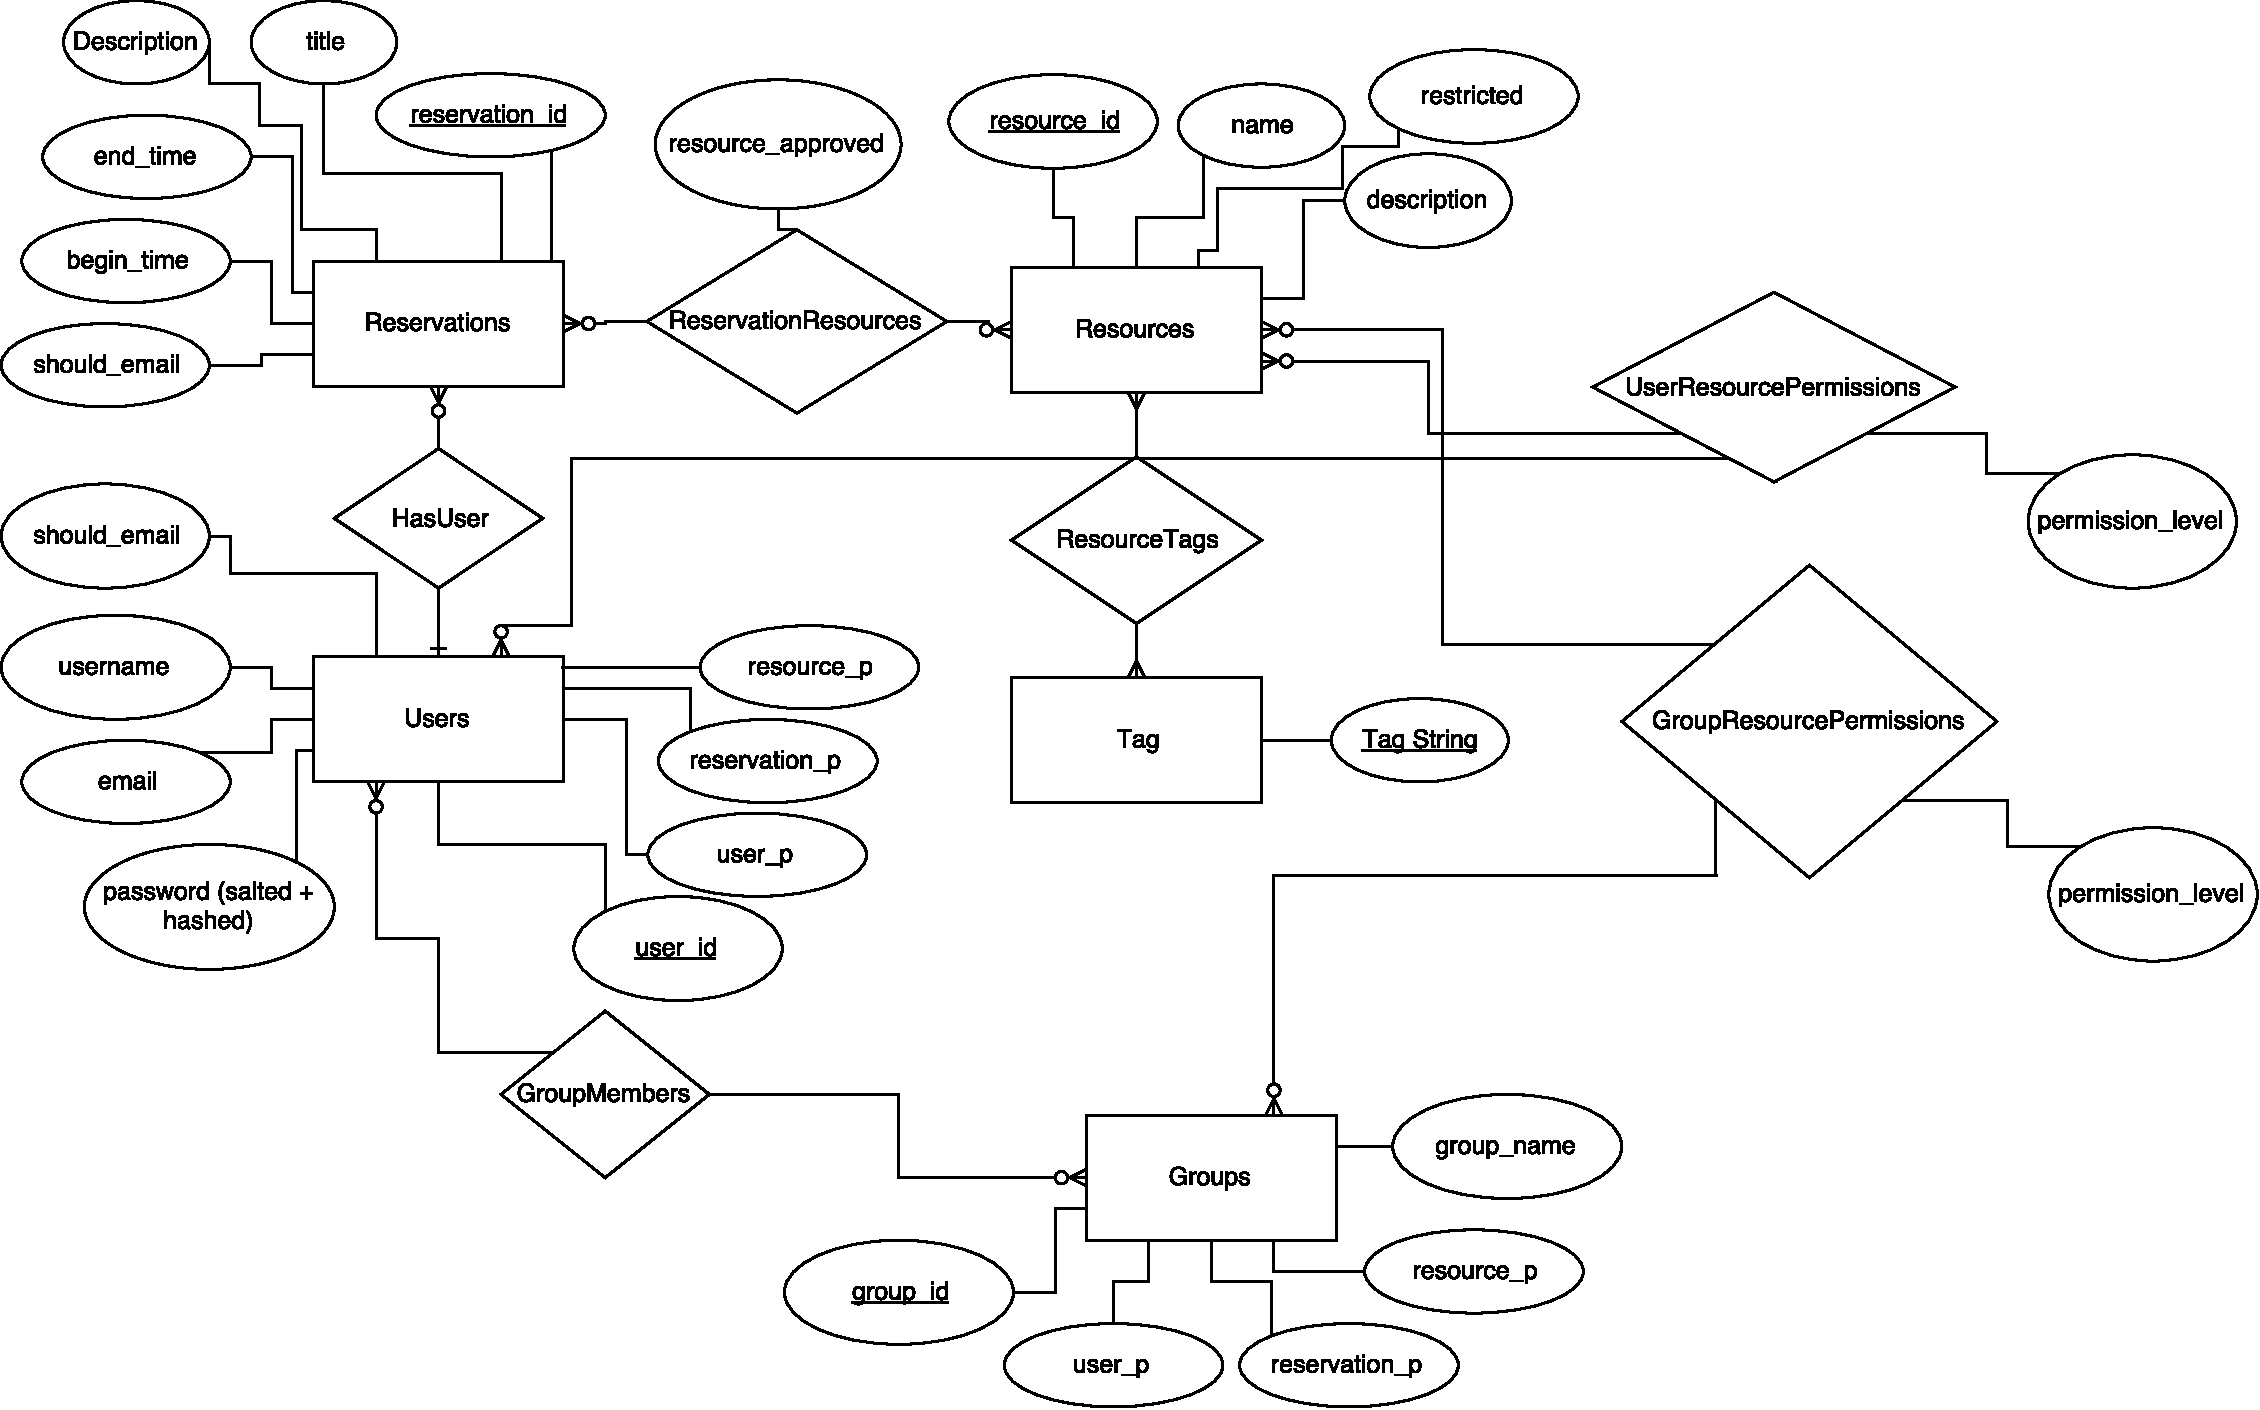
\includegraphics[height=4in]{Evolution3DB.pdf}
\end{center}
\caption{DB Schema}
\end{figure}

\end{document}